\documentclass[review]{elsarticle}

\usepackage{lineno,hyperref,amsmath,amsfonts,amssymb,graphicx}
\modulolinenumbers[5]

%\journal{Journal of \LaTeX\ Templates}

%%%%%%%%%%%%%%%%%%%%%%%
%% Elsevier bibliography styles
%%%%%%%%%%%%%%%%%%%%%%%
%% To change the style, put a % in front of the second line of the current style and
%% remove the % from the second line of the style you would like to use.
%%%%%%%%%%%%%%%%%%%%%%%

%% Numbered
%\bibliographystyle{model1-num-names}

%% Numbered without titles
%\bibliographystyle{model1a-num-names}

%% Harvard
%\bibliographystyle{model2-names.bst}\biboptions{authoryear}

%% Vancouver numbered
%\usepackage{numcompress}\bibliographystyle{model3-num-names}

%% Vancouver name/year
%\usepackage{numcompress}\bibliographystyle{model4-names}\biboptions{authoryear}

%% APA style
%\bibliographystyle{model5-names}\biboptions{authoryear}

%% AMA style
%\usepackage{numcompress}\bibliographystyle{model6-num-names}

%% `Elsevier LaTeX' style
\bibliographystyle{elsarticle-num}
%%%%%%%%%%%%%%%%%%%%%%%

%\usepackage[linesnumbered,ruled,vlined]{algorithm2e}
\usepackage[linesnumbered, ruled, vlined]{algorithm2e}
\SetKwInput{KwInput}{Input}                % Set the Input
\SetKwInput{KwOutput}{Output}              % set the Output

\newtheorem{definition}{Definition}

\begin{document}

\begin{frontmatter}

\title{Generalized Critic: An Ensemble-Based Value Approximation for Actor-Critic Deep Reinforcement Learning}

%% or include affiliations in footnotes:
%\author[hbn]{Roumeissa Kitouni}
%\cortext[mycorrespondingauthor]{Corresponding author}
%\ead{r.kitouni@hit.edu.cn}

%\author[cne]{Abderrahim Kitouni}
%\ead{a.kitouni@gmail.com}

%\author[hbn]{Feng Jiang}
%\ead{fjiant@hit.edu.cn}

%\address[hbn]{Harbin Institute of Technology, 92 Xidazhi Street, Nangang District, Harbin City, Heilongjiang Province, China}
%\address[cne]{Université frères Mentouri Constantine 1, route d'Ain El Bey, 25017 Constantine, Algeria}

\begin{abstract}
We present a general model for actor-critic policy gradient methods with Ensemble models, and test an example implementation on four robotic environments.
The source code implementing the present work as well as the experiment logs presented in section \ref{sec:exp} can be consulted and accessed online\footnote{https://github.com/syrma/GC\_paper}.
\end{abstract}

\begin{keyword}
deep reinforcement learning \sep actor critic \sep policy optimization \sep ensemble learning \sep continuous control \sep generalization \sep model-free
\end{keyword}


\end{frontmatter}

\section{Introduction}

In the recent years, technical advancement gave Artificial intelligence (AI) a new breath by facilitating the use of computation-heavy, highly scalable Artificial Neural Networks (ANN) as function approximators, thus achieving remarkable results in what is commonly referred to as Deep Learning. Indeed, despite their theoretical simplicity, ANNs have proved to be a reliable tool to approximate complex, real-world functions given enough computational power. Deep Reinforcement Learning refers to the practice of harnessing the combined power of new technologies and deep ANNs to put into practice the previously purely theoretical methods of Reinforcement Learning (RL). 

Deep RL subsequently achieved impressive results, in particular in board games such as Go, Shogi and Chess, leading to the algorithm largely outperforming any human player. In several more cases however, Deep RL offers more potential for future AI research than tangible state-of-the-art results. For instance, Reinforcement Learning methods have yet to be used in physical systems, either due to their needing far too much data to learn from %TODO (reference to some review of dqn or vpg)
or to their complexity and sensitivity to hyperparameters. %TODO (reference to drl that matters and similar stuff). 
While many applications are still more reliably solved with the help of human-expert-labeled data %ref
RL research offers the possibility of AI eventually growing beyond the need for such data, doing so by working on two fronts:
\begin{itemize}
\item Equipping AI with the autonomy to generate its own learning examples through interaction with the environment, instead of relying on expert-labeled data.
\item Developing a meta-paradigm that solves the problem of learning, irrespective of the task or application to be learned.
\end{itemize}


%\section{Related Works}
\label{sec:rw}

There have been many efforts to reduce the high variance associated with these algorithms to make them more sample-efficient.

\subsection{Generalization and performance optimization for PPO}

\subsection{Ensemble methods in Reinforcement Learning}

\section{Preliminaries}
\label{sec:prelim}
This work builds on past theory on Reinforcement Learning and Policy Gradients. In this section, we will briefly summarize the essential structure of the RL problem and the categories of solutions relevant to the context of the present work.

\subsection{Markov Decision Processes}

Reinforcement Learning is the field of Machine Learning concerned with decision making within an uncertain environment, acting upon it through actions with uncertain consequences, with the aim of achieving a specific goal while maximizing a numerical reward. A distinguishing feature of RL is that the agent interacts with the environment and pieces together a policy $\pi_theta$—the solution to the problem relying purely on the feedback of the environment with no input from human experts in any form. 

It is possible to model virtually any problem that corresponds to the description above using a mathematical framework called a Markov Decision Process (MDP.) 

The MDP is defined by the tuple ($\mathcal{S}, \mathcal{A}, \mathcal{P}, r, \rho_0$) where $\mathcal{S}$ is the set of states, $\mathcal{A}$ is the set of actions, $\mathcal{P}: \mathcal{S}\times\mathcal{A}\times\mathcal{S}\mapsto \mathbb{R}$ is the transition probability distribution, $r: \mathcal{S}\times\mathcal{A}\times\mathcal{S} \mapsto \mathbb{R}$ is the reward function, and $\rho_0:\mathcal{S}\mapsto\mathbb{R}$ is the initial state distribution.


\subsection{Proximal Policy Optimization}

PPO (Proximal Policy Optimization\cite{schulman2017proximal}) is one of the most popular Deep RL algorithms, which has since been applied to a wide range of domains from robotics\cite{andrychowicz2020learning} to chip design\cite{mirhoseini2021graph}. It is a comparatively accessible algorithm to implement and deploy. A trend in model-free RL has been to improve performance through increasingly complex methods, which comes at the great cost of making RL methods hard to reproduce and validate as well as unpractical to use in physical systems. This is at odds with the very purpose of advancing Reinforcement Learning research, a field aiming to create a general paradigm that requires less human intervention than any other conventional Artificial Intelligence paradigm. 


\section{Method}
\label{sec:meth}
\begin{algorithm}[H]
\DontPrintSemicolon
  
  \KwInput{Initial actor network parameters $\theta_0$, initial critic parameter list $\phi^0_0, \dots, \phi^n_0$}
  %\KwOutput{Your output}
  %\KwData{Testing set $x$}
  $\sum_{i=1}^{\infty} := 0$

  \tcc{Now this is an if...else conditional loop}
  \For{i in [1, epochs]}{     
\For{i in [1, size]}{     
         Run $\pi_{\theta_{old}}$ collect set of trajectories $\mathcal{D}_k$
   }
   }

   Compute $\hat{V}$

   Compute GAE

   Compute the policy loss and update the policy via gradient ascent

  \For{i in [1, n]}
    {
    	Update $V_{\phi^1}$	
    } 
    
\caption{Generalized Critic Policy Optimization}

\end{algorithm}

\begin{figure}[!htb]
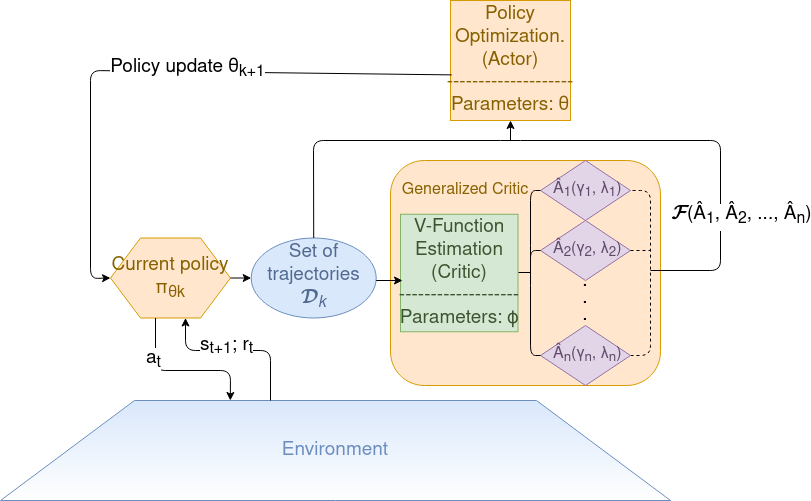
\includegraphics[width=\linewidth]{images/model}
\caption{Policy update scenario with a generalized critic.}
\label{fig:model}
\end{figure}


\section{Experiments}
\label{sec:exp}
	To illustrate the potential of the theoretical model presented in section 3, we implemented an example to analyze the practical aspect as well as the empirical results.

In this section, we will proceed to describe our experimental settings, explain choices related to the implementation, and present the resulting data as well as the conclusions we draw from them.

\subsection{Experimental Setting}

\subsubsection{Code-level optimizations}

A group of code-level optimizations have been identified and compiled by previous work \cite{engstrom2020implementation}\cite{shengyi2022the37implementation} in an effort to reproduce reported results for the PPO algorithm. 

It is worth  noting that while none of these optimizations are formally included in the basic definition of the algorithm or credited for its performance, some of them are a de-facto part of any functional implementation, especially those that relate to compatibility with  continuous space environments. The rest are not strictly required for the algorithm to function. Nonetheless, they are needed to reproduce the state-of-the-art results and are, as a rule, included in benchmark implementations \cite{huang2021cleanrl} \cite{baselines}. %cite baselines and cleanrl

Due to the ill-defined nature of what constitutes a baseline for PPO or what degree of optimization still falls within the scope of the algorithm, we have elected to implement and run a minimalist interpretation of the algorithm with only enough optimizations to be functional and to support the environments we test on. We used the Keras library to implement the neural networks and their optimizations.

This implementation does not therefore reproduce the highest reported results for PPO, as the purpose of this research is to establish the effect of our contribution by comparison to a similar basis that does not implement it.

Following are the optimizations and the main reason for their inclusion:

\begin{description}
\item[Support for continuous action space environments] %(mean and std as output instead of logits(??))
\item[Advantage normalization] while this optimization does not improve the final performance\cite{andrychowicz2020learning}
%Advantage norm essentially doesn't make your gradients go insane, and you also get an equal number of positive gradients to negative gradients, making your policy weights not go insane (which is why you tend to see more stable training) But at the tail end of training, if your algo is stable 'enough', the gradients at the end of training are really miniscule anyway, and do nothing to improve final performance
\item[Reward scaling] We divide the rewards by the (estimated) standard deviation of the discounted cumulative rewards at step $t$ by a factor $\gamma$: $R_t = \sum_{i=0}^t \gamma^{t-i} r_i$. %This optimization was only used for training on the Hopper task.
\item[KL fallback] Approximates the Kullback-Leibler (KL) divergence and cancels a policy update if the value is above a threshold. Implemented to prevent catastrophic unlearning\cite{dossa2021empirical}, a phenomenon observed in PPO where a suboptimal update causes the average episodic reward to drop brusquely and never recover.
\end{description}

\subsubsection{Testing Setup}

Our experiment setting consists of four robotic tasks from the Pybullet suite of environments using Gym. Gym\cite{brockman2016openai} is an open source toolkit for RL research initially released by OpenAI. 

We run the algorithm on the four continuous tasks with different settings (baseline PPO, PPO with Generalized Critic, PPO with Generalized Critic + bootstrap). We run each configuration over 10 random seeds and track the recorded returns using Weights and Biases\cite{wandb}

For each of the critics, we estimate the advantage function using the Generalized Advantage Estimation method\cite{schulman2015highdimensional}.
The hyperparameters are detailed in table %\ref{hyperparameters}

\begin{table}
  \begin{center}
    \begin{tabular}{cc}
      \hline 
      hyperparameter & value \\ 
      \hline 
      \verb!total timesteps! & \verb!2M! \\
      \verb!PPO update iterations per epoch! &  \verb!80! \\
      \verb!GAE gamma! & \verb!0.99! \\
      \verb!GAE lambda! & \verb!0.97! \\
      \verb!kl_target! & \verb!0.1! \\
      \verb!policy network hidden layers! & \verb![120, 84]! \\
      \verb!(policy network) learning_rate! & \verb!3e-4! \\
      \verb!(policy network) activation function! & \verb!relu!\\
      \verb!value network hidden layers! & \verb![64]! \\
      \verb!(value network) learning_rate! & \verb!3e-4! \\
      \verb!(value network) activation function! & \verb!relu! \\
      \hline      
    \end{tabular}
  \end{center}
  \caption{Experiment hyperparameters and their values}
  \label{hyperparameters}
\end{table}




\subsubsection{Experiment tracking}
 



%Good for Hopper
% Meh for Humanoid
% bad for hc? smth bl3t

\subsection{Experimental Results and Analysis}


\begin{figure}[!htb]

\begin{minipage}[b]{.5\linewidth}
  \centering
  \centerline{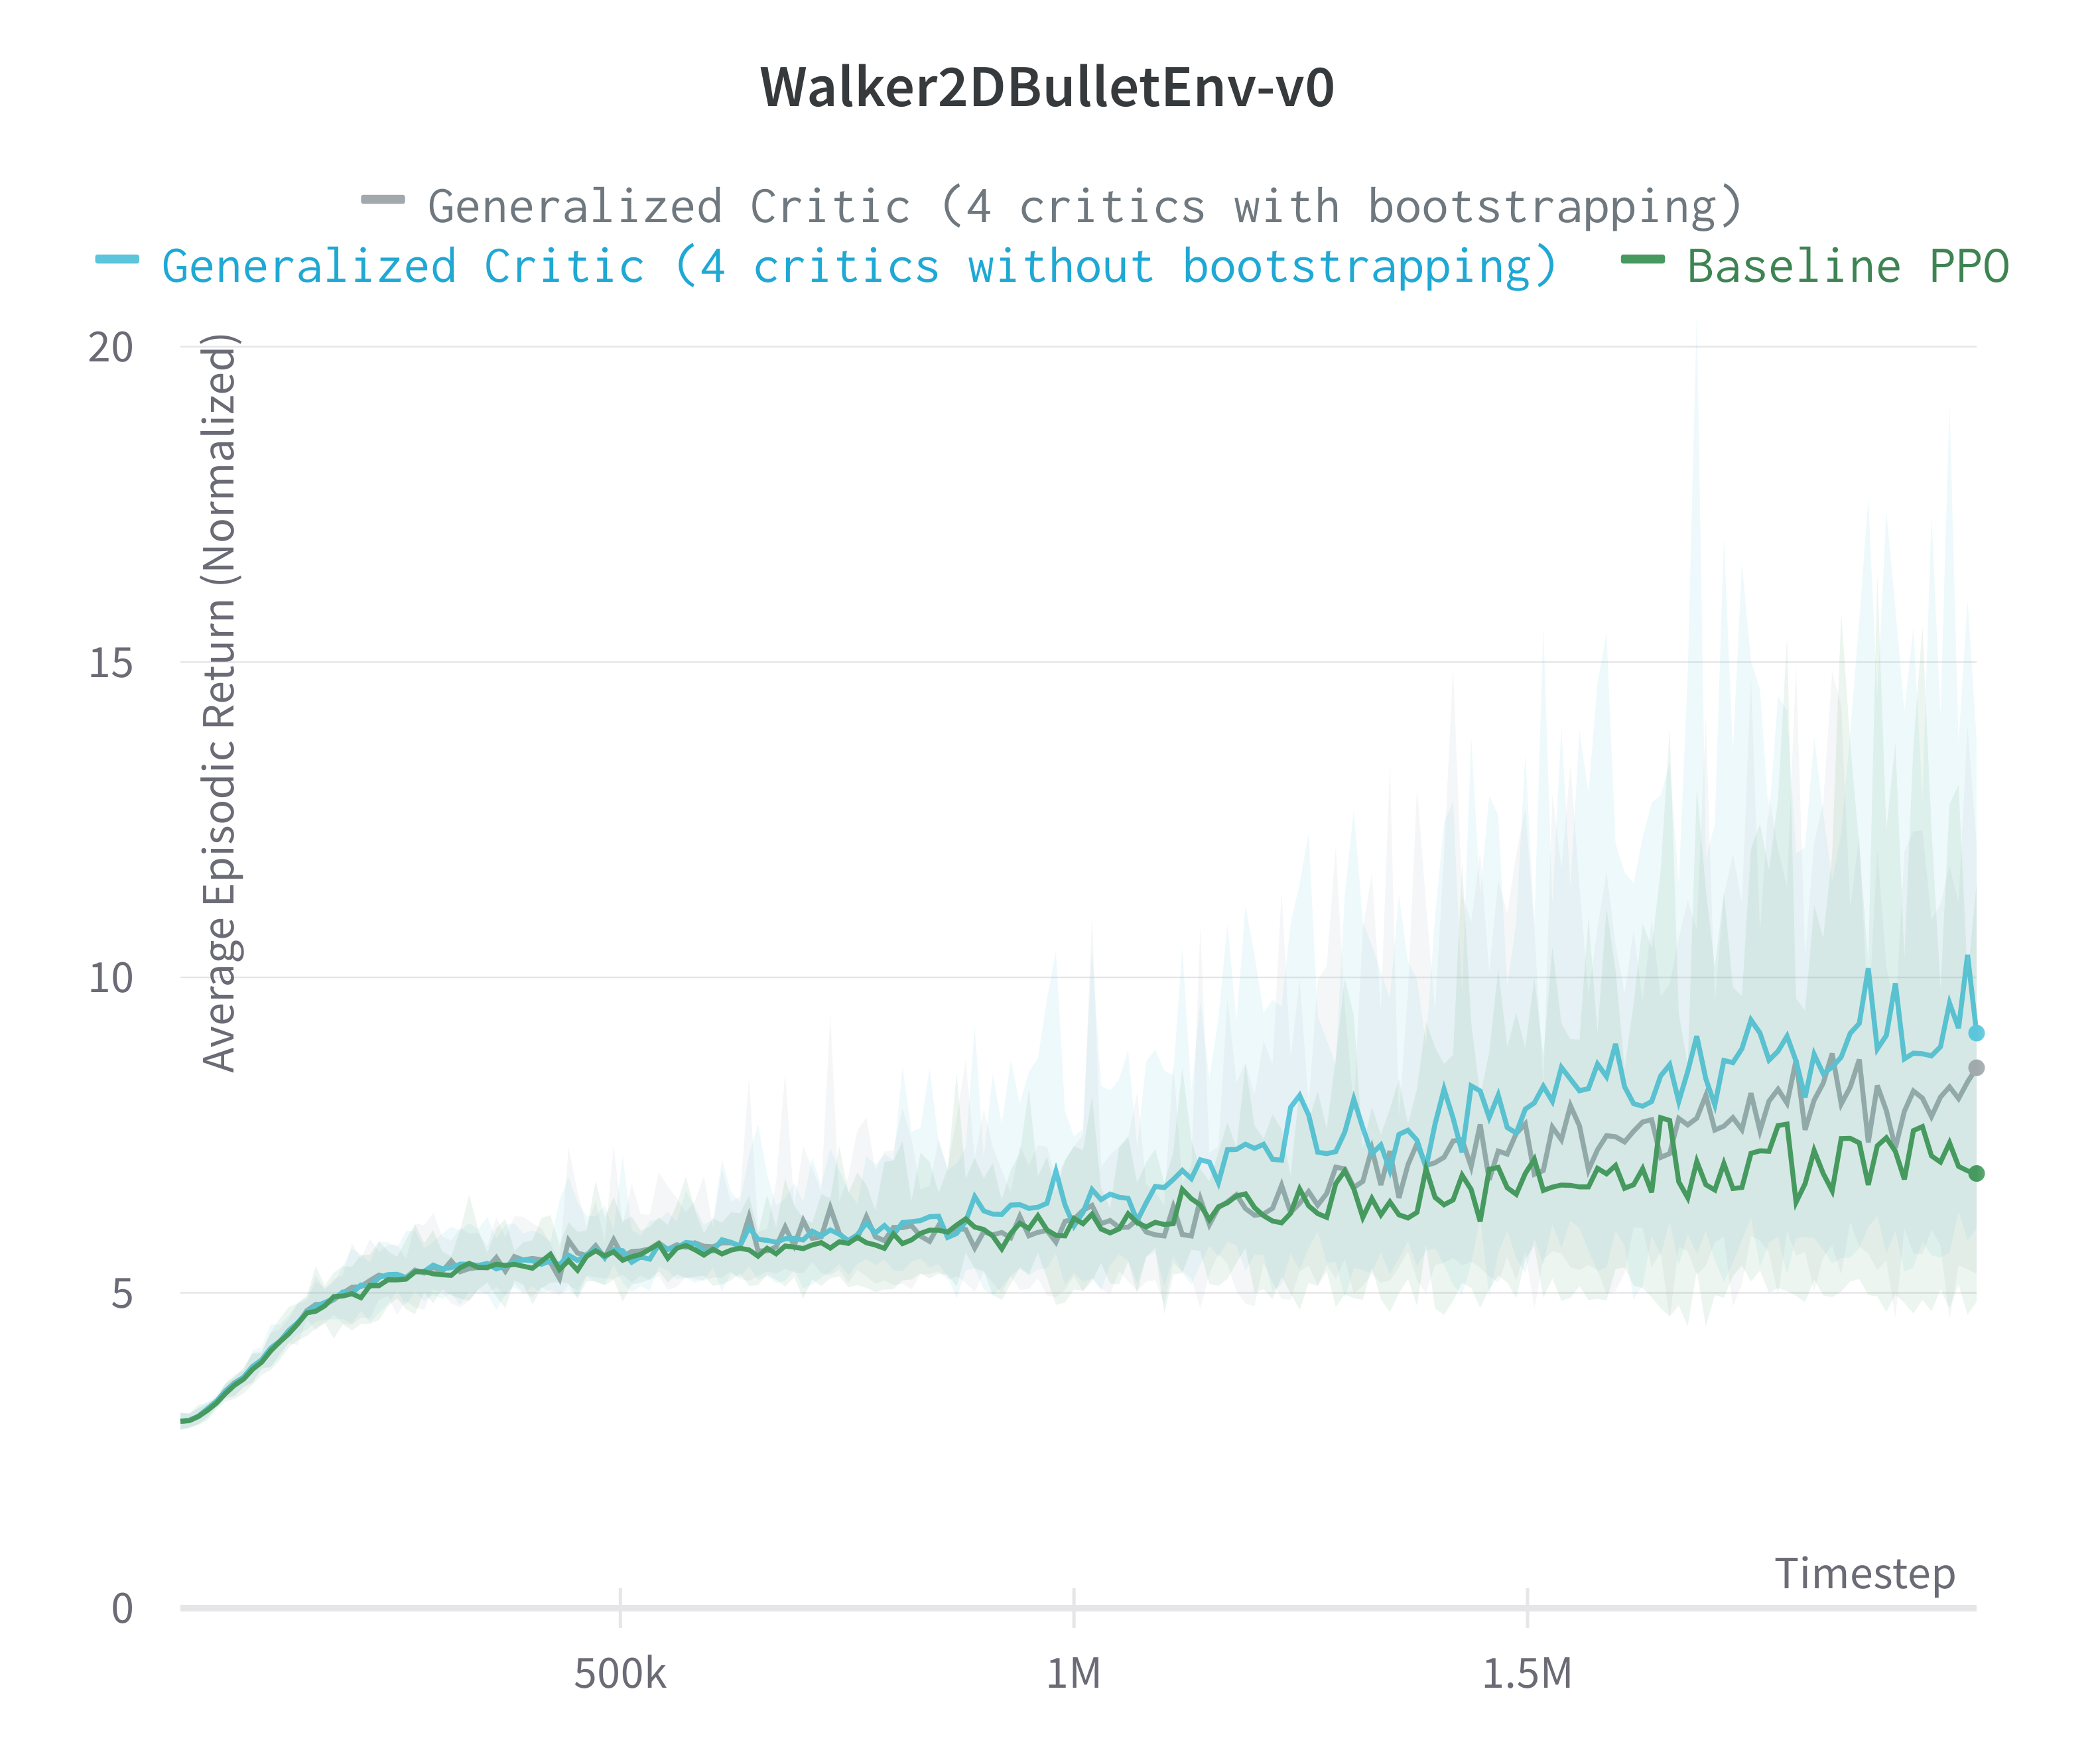
\includegraphics[width=\linewidth]{images/walker2D}}
%  \vspace{2.0cm}
%  \centerline{(a) Walker2DBulletEnv-v0}\medskip
\end{minipage}
\begin{minipage}[b]{.5\linewidth}
  \centering
  \centerline{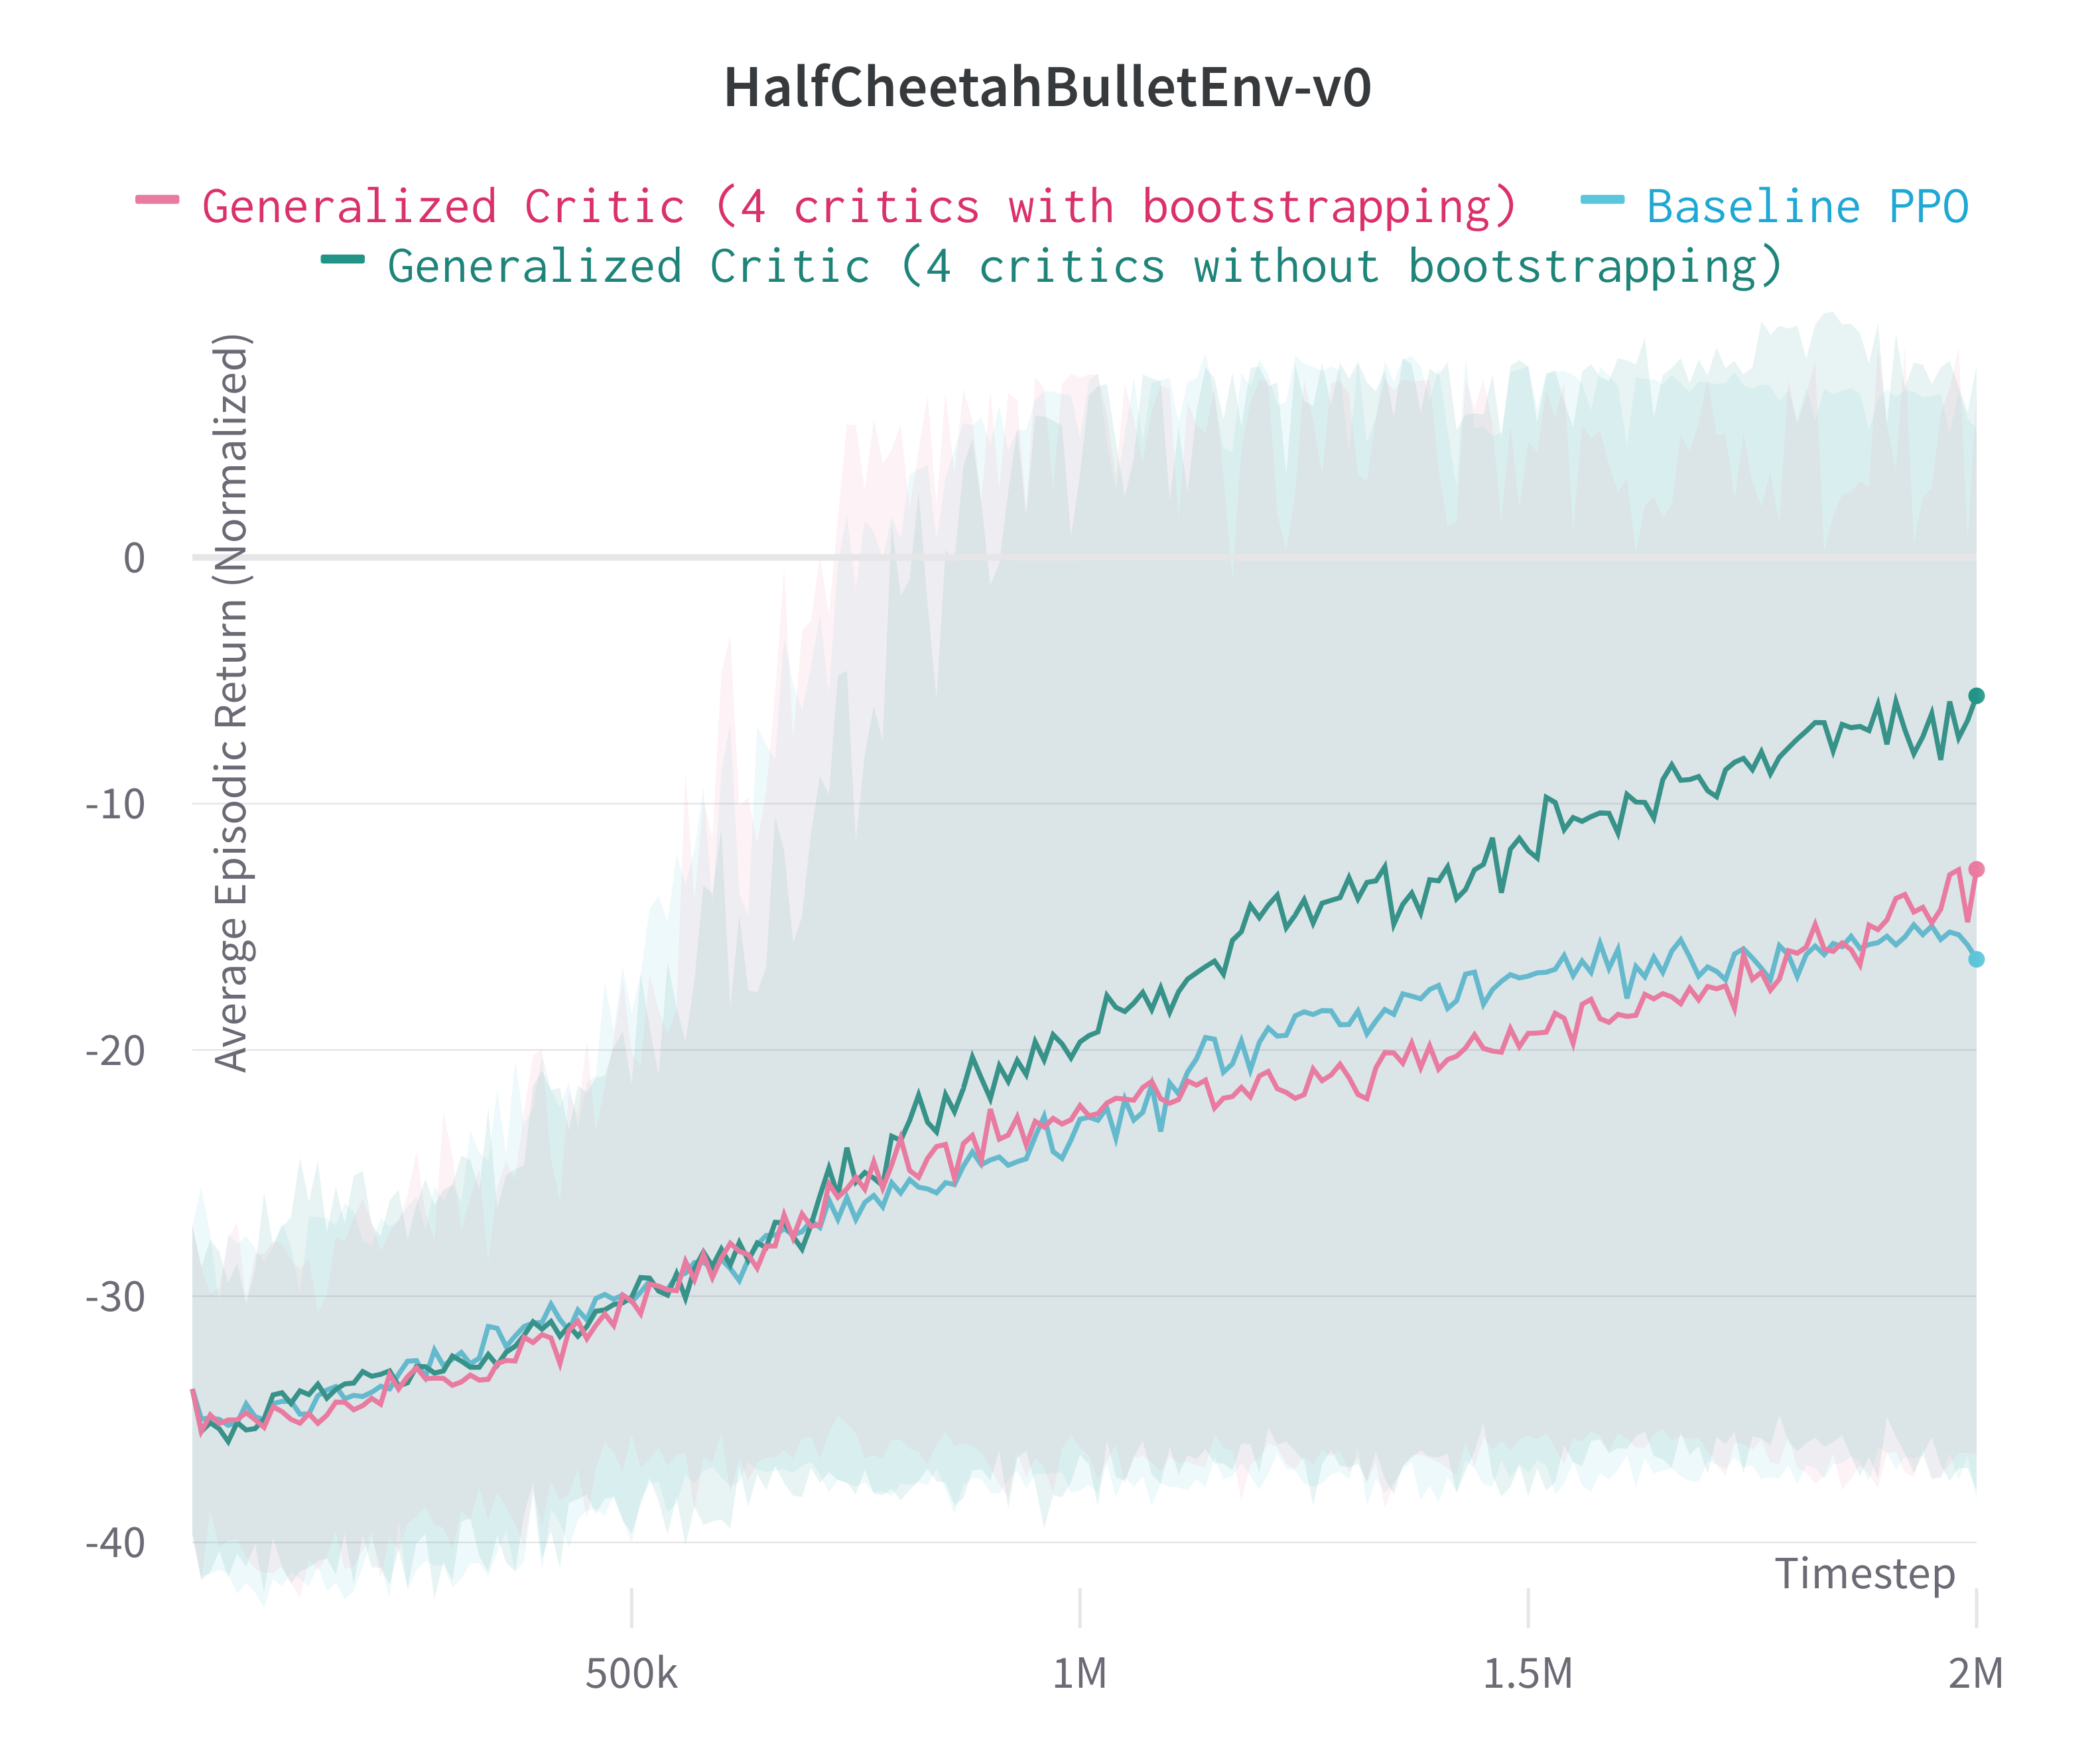
\includegraphics[width=\linewidth]{images/halfcheetah}}
%  \vspace{2.0cm}
%  \centerline{(b) HalfCheetahBulletEnv-v0}\medskip
\end{minipage}

\begin{minipage}[b]{.5\linewidth}
  \centering
  \centerline{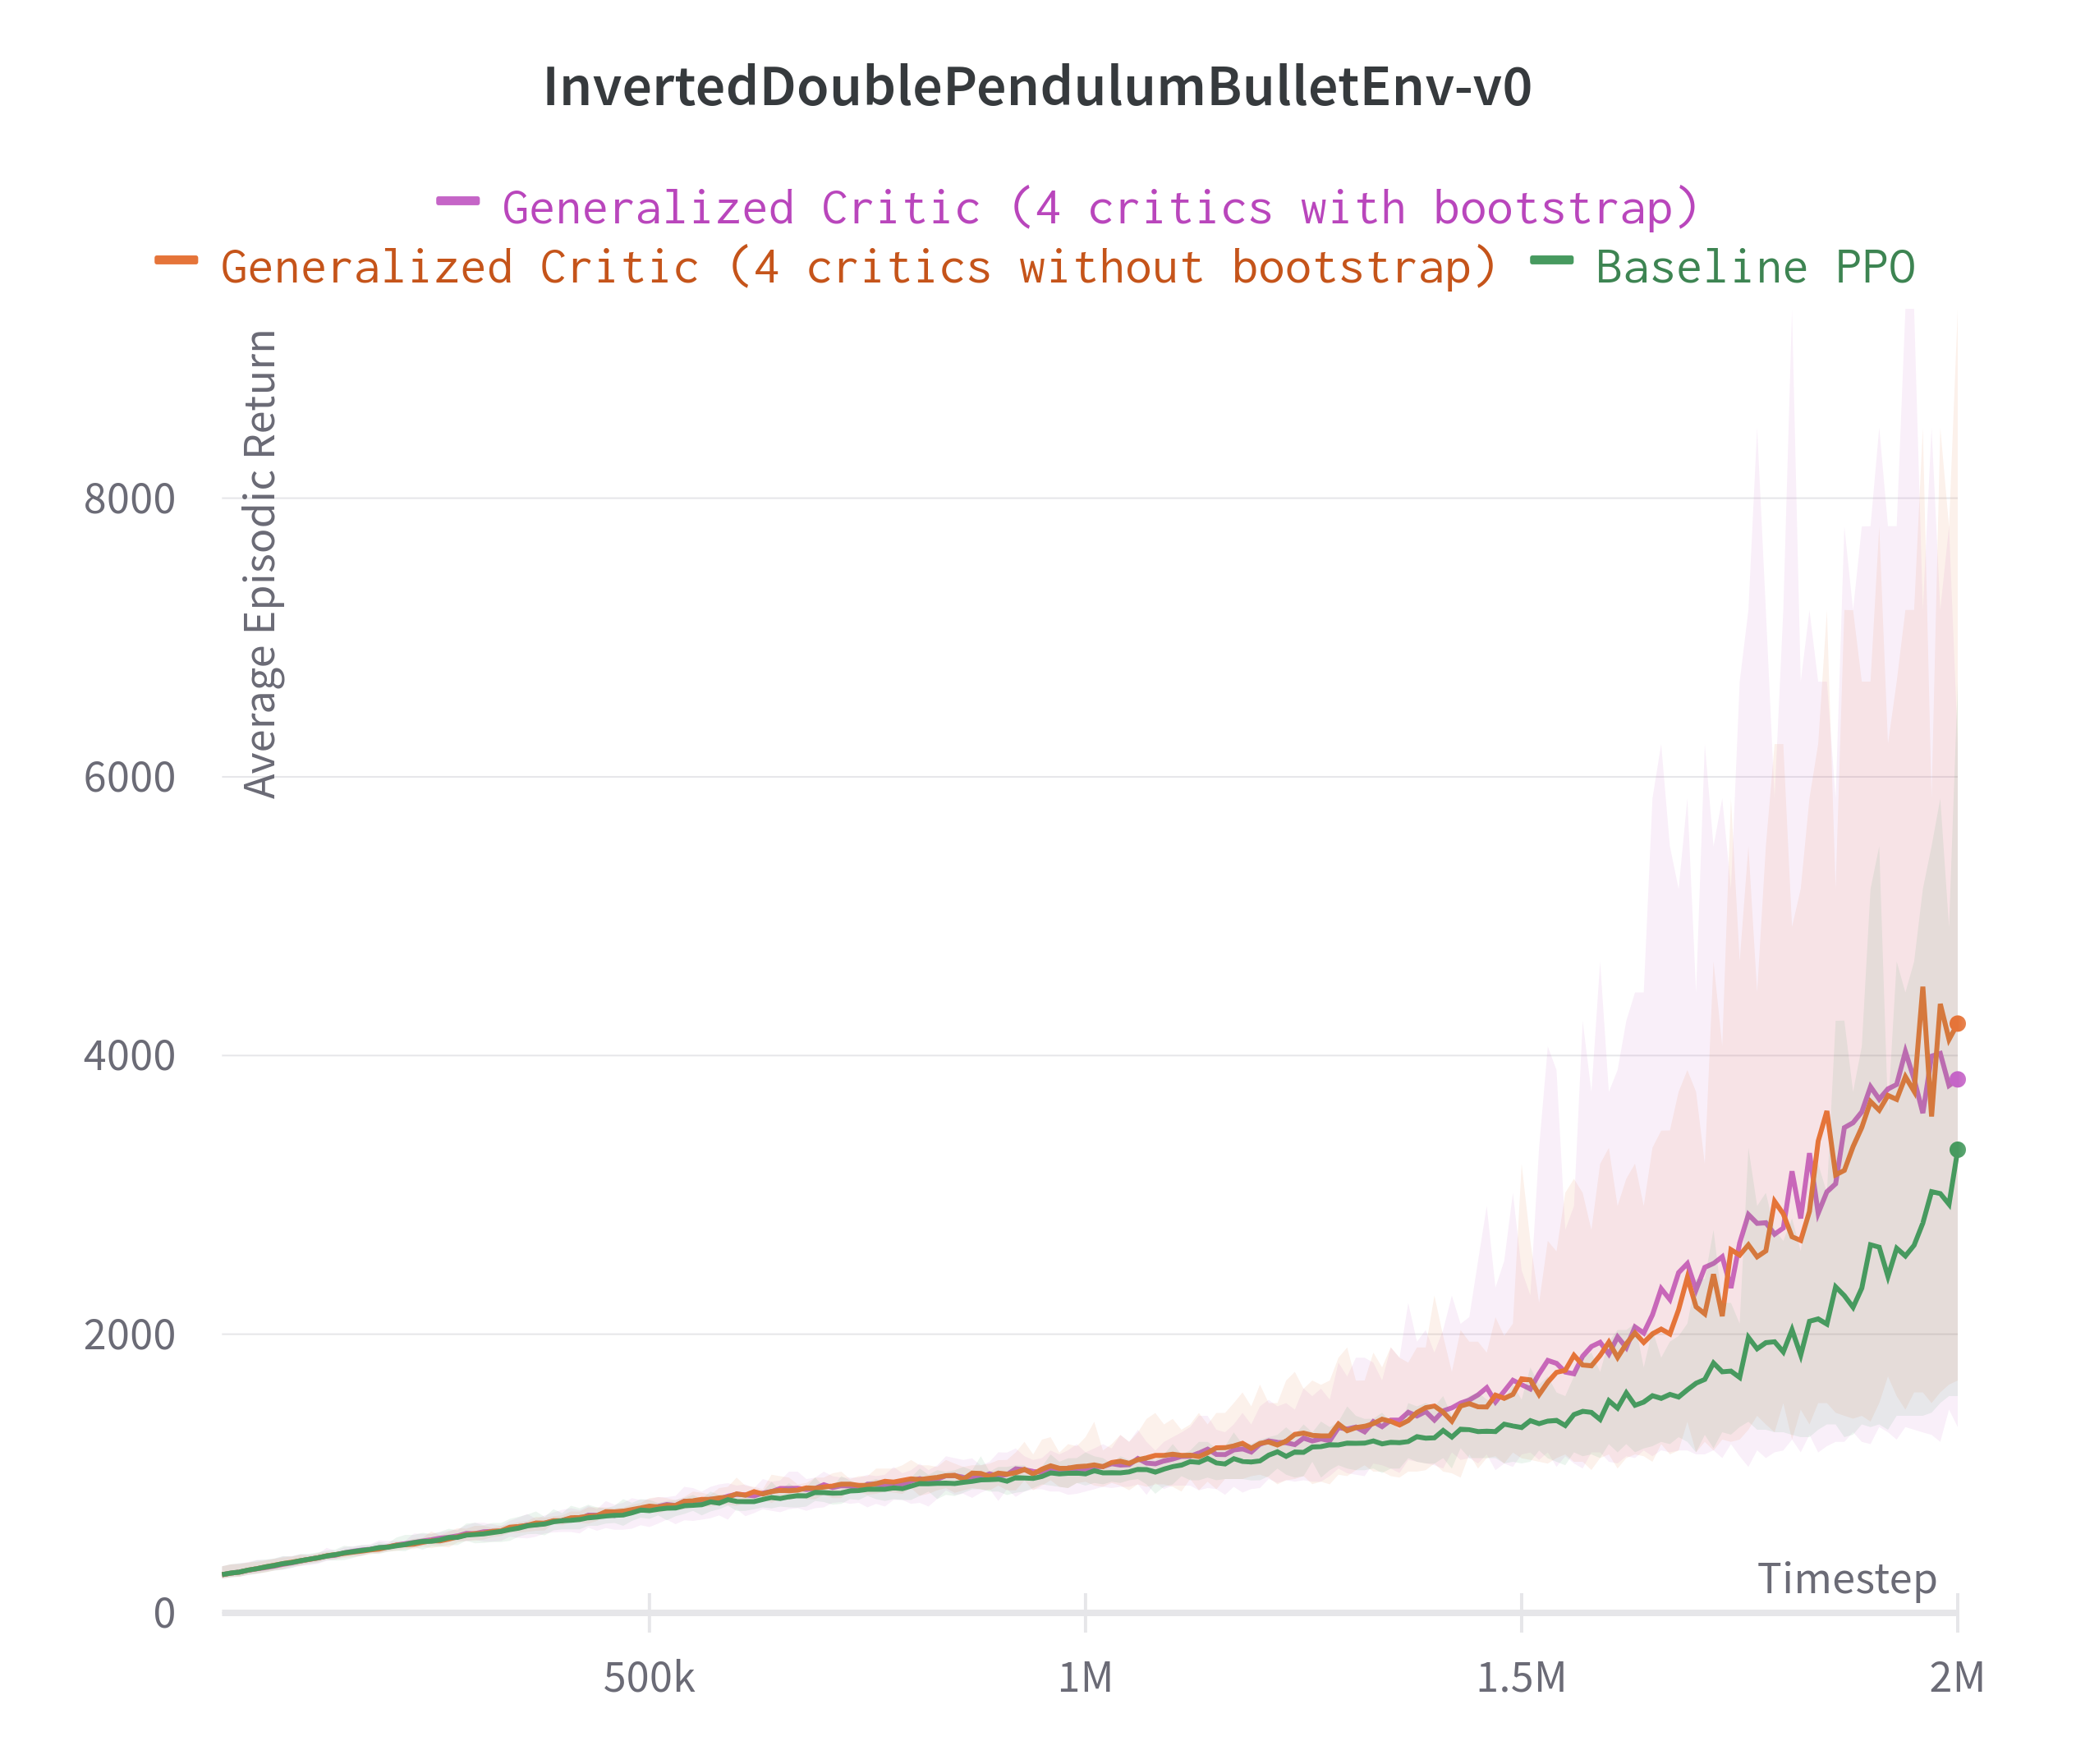
\includegraphics[width=\linewidth]{images/inverteddoublependulum}}
%  \vspace{2.0cm}
%  \centerline{(a) InvertedDoublePendulumBulletEnv-v0}\medskip
\end{minipage}
\begin{minipage}[b]{.5\linewidth}
  \centering
  \centerline{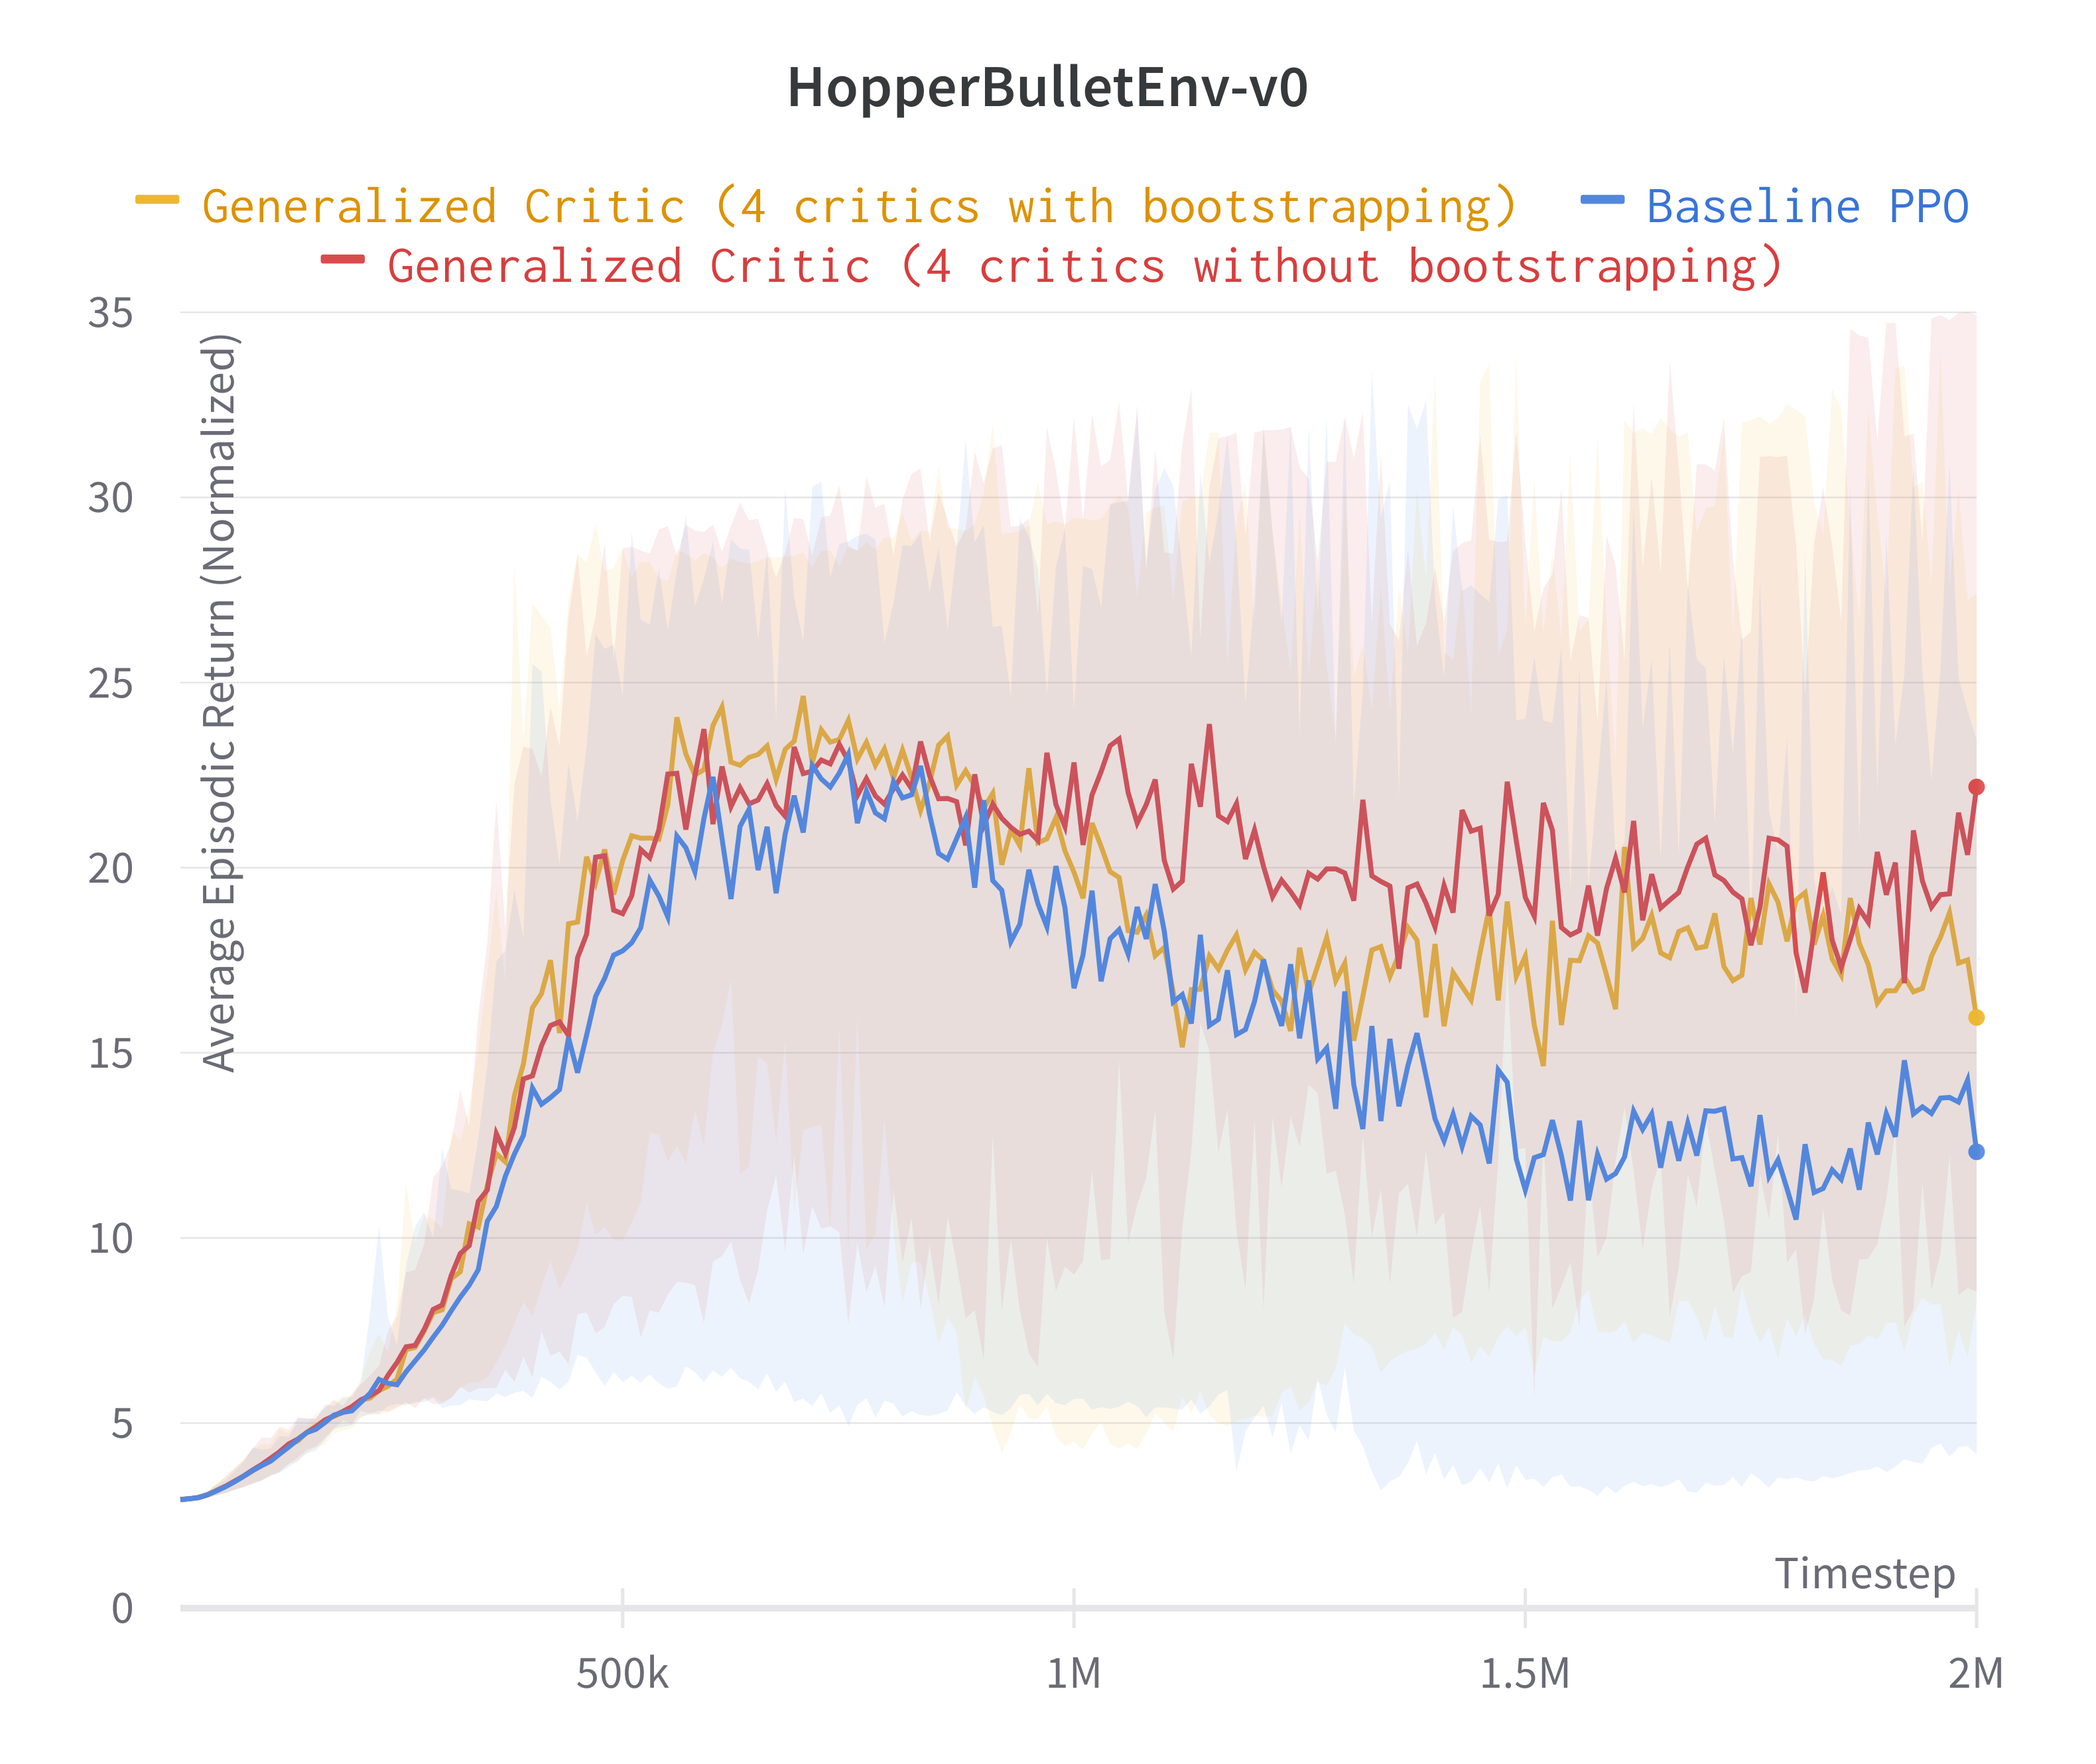
\includegraphics[width=\linewidth]{images/hopper}}
%  \vspace{2.0cm}
%  \centerline{(b) HopperBulletEnv-v0}\medskip
\end{minipage}
\caption{(2)}
\label{exp2}
\end{figure}


\section{Conclusion}
\label{sec:conc}
We have presented a general model for critics in Actor-Critic methods. We believe that this representation can become a basis to simplify the design of complex deep reinforcement learning agents.

We have provided a basic, practical example of exploiting the model to design a practical method and test it against currently challenging state-of-the-art control tasks.

As a future research perspective, we aim to provide a more complete set of experiments, in particular: 
\begin{itemize}
\item thoroughly investigate the range of possible hyperparameters and deduce a more general use case;
\item represent the aggregation function with different models, including trained nonlinear approximators;
\item encompass more known policy optimization methods and algorithms, and adapt our method accordingly.
\end{itemize}

In addition to these pratical considerations, we intend to study the Generalized Critic model's shortcomings and provide more formal representations.




% -------------------------------------------------------------------------
\bibliography{mybibfile}

\end{document}
